\chapter{Documento de Requisitos}\label{cap:06requisitos}

\section{Introducción}




%R.I%%%%%%%%%%%%%%%%%%%%%%%%%%%%%%%%%%%%%%%%%%%%%%%%%%%%%%%%%%%%%%%%%%%%%
%\section{Requisitos de Información}


%R.F%%%%%%%%%%%%%%%%%%%%%%%%%%%%%%%%%%%%%%%%%%%%%%%%%%%%%%%%%%%%%%%%%%%%%
\section{Requisitos funcionales}

\subsection{Diagrama de casos de uso} \label{subsec:06FRdiagrama}

\begin{figure}[H]
    \centering
    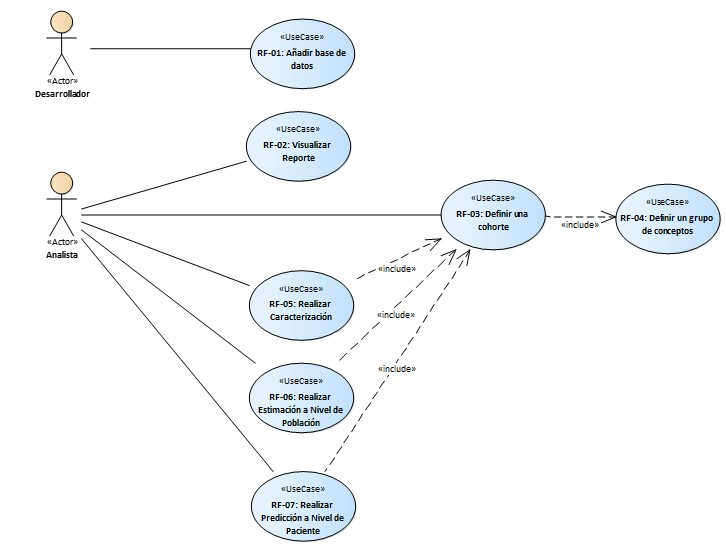
\includegraphics[width=0.90\textwidth]{figures/FRdiagram.jpg}
    \caption{Diagrama de casos de uso}
    \label{fig:FRdiagram}
\end{figure}

\subsection{Casos de uso del sistema}

\begin{figure}[H]
    \centering
    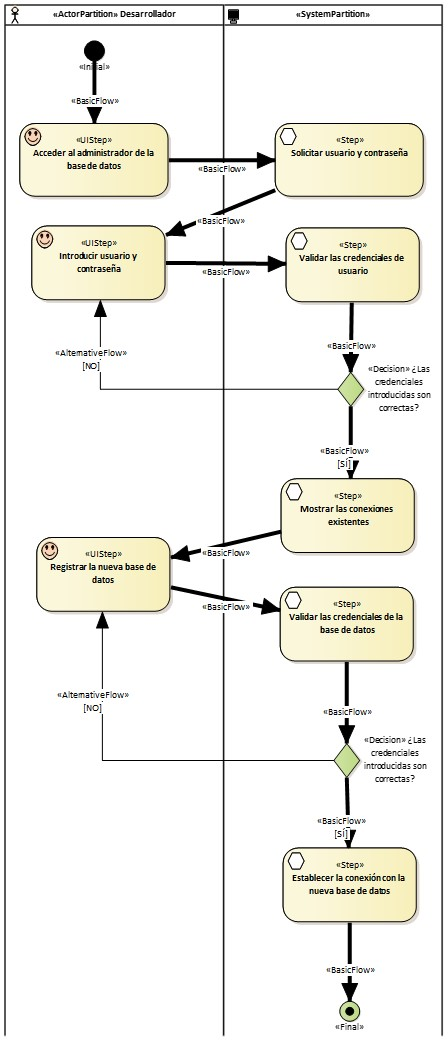
\includegraphics[width=0.60\textwidth]{figures/FR01.jpg}
    \caption{Diagrama de actividad de RF-01:Añadir base de datos}
    \label{fig:FR01}
\end{figure}

\begin{figure}[H]
    \centering
    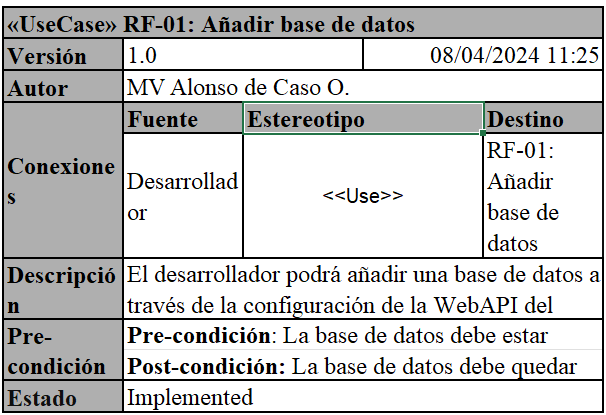
\includegraphics[width=0.65\textwidth]{tables/RF01tab.png}
    \captionof{table}{Caso de uso de RF-01:Añadir base de datos}
    \label{table:RF01tab}
\end{figure}

\begin{figure}[H]
    \centering
    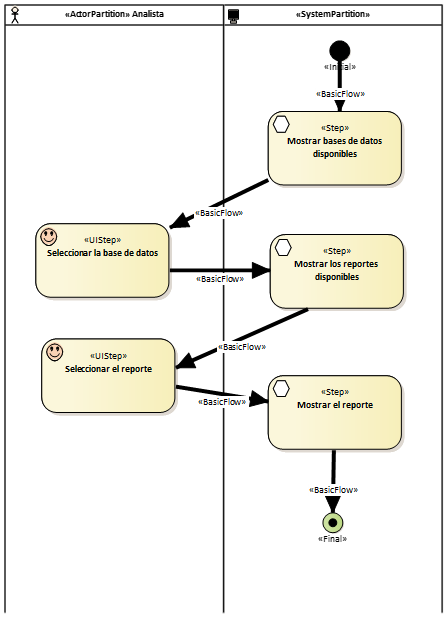
\includegraphics[width=0.65\textwidth]{figures/FR02.png}
    \caption{Diagrama de actividad de RF-02: Visualizar Reporte}
    \label{fig:FR02}
\end{figure}

\begin{figure}[H]
    \centering
    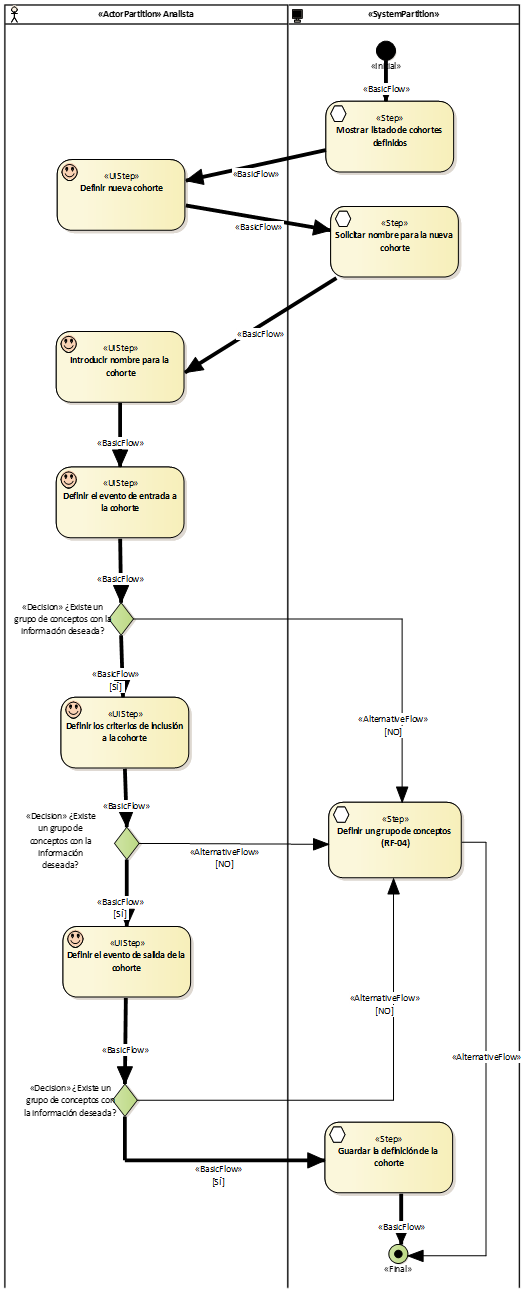
\includegraphics[width=0.65\textwidth]{figures/FR03.png}
    \caption{Diagrama de actividad de RF-03: Definir una cohorte}
    \label{fig:FR03}
\end{figure}

\begin{figure}[H]
    \centering
    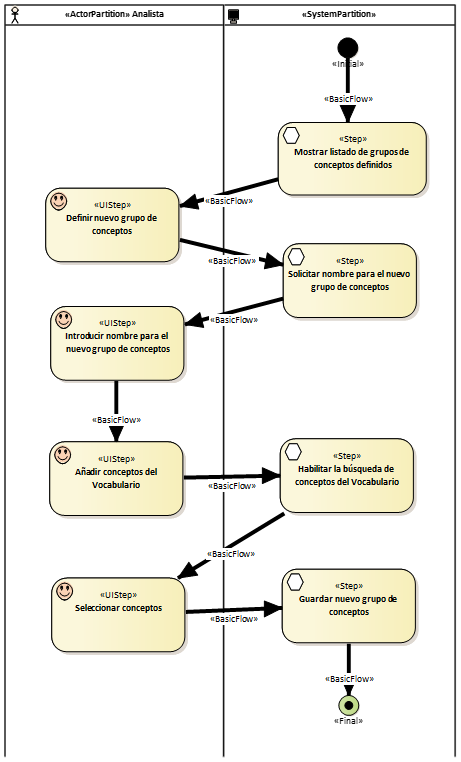
\includegraphics[width=0.65\textwidth]{figures/FR04.png}
    \caption{Diagrama de actividad de RF-04: Definir un grupo de conceptos}
    \label{fig:FR04}
\end{figure}

\begin{figure}[H]
    \centering
    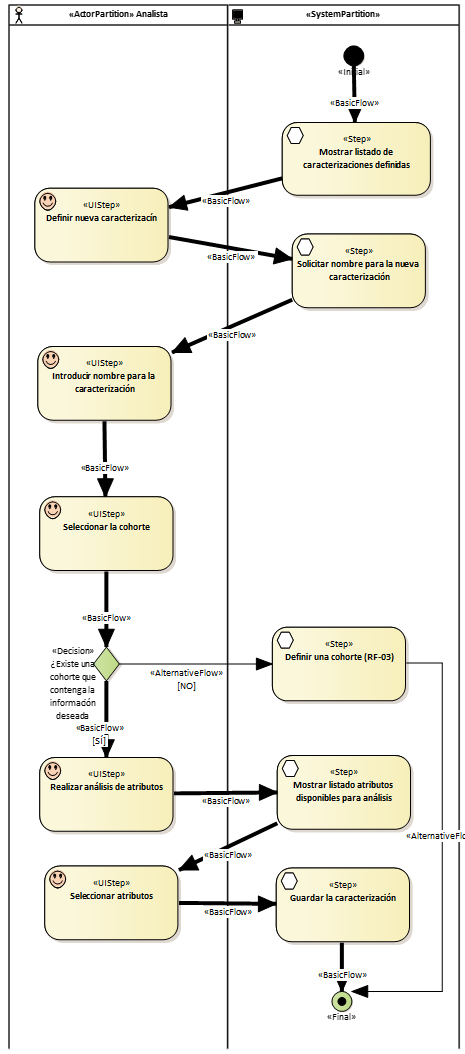
\includegraphics[width=0.65\textwidth]{figures/FR05.png}
    \caption{Diagrama de actividad de RF-05: Realizar Caracterización}
    \label{fig:FR05}
\end{figure}

\begin{figure}[H]
    \centering
    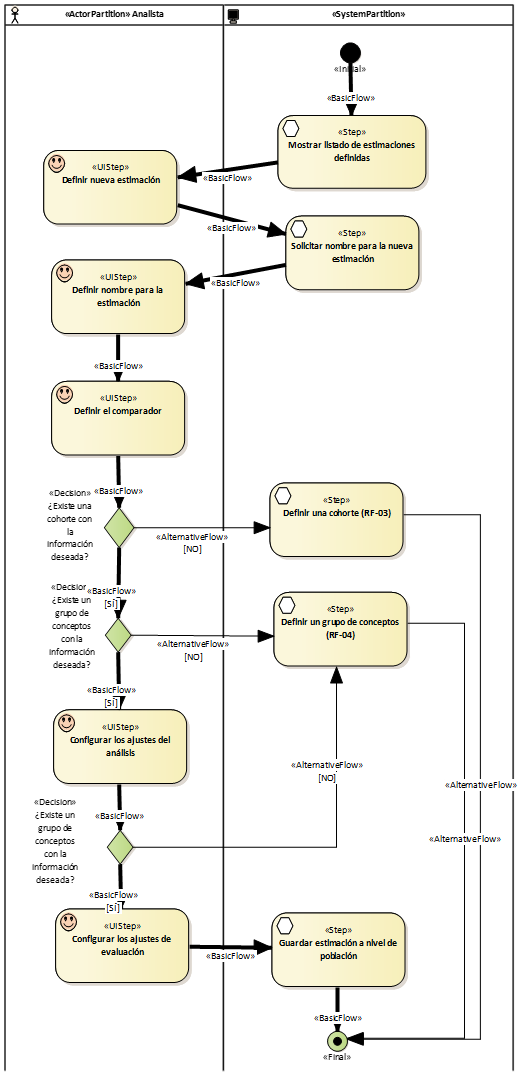
\includegraphics[width=0.65\textwidth]{figures/FR06.png}
    \caption{Diagrama de actividad de RF-06: Realizar Estimación a nivel de Población}
    \label{fig:FR06}
\end{figure}

\begin{figure}[H]
    \centering
    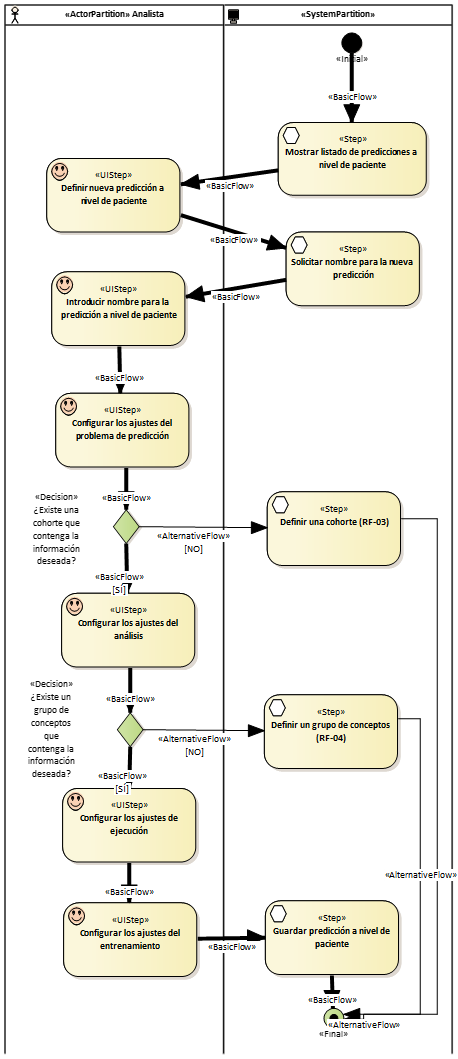
\includegraphics[width=0.65\textwidth]{figures/FR07.png}
    \caption{Diagrama de actividad de RF-07: Realizar Predicción a nivel de Paciente}
    \label{fig:FR07}
\end{figure}


\section{Requisitos no funcionales}


\section{Conclusiones}

En este capítulo concluimos que...
